%----------------------------------------------------------------------------------------
%	DOCUMENT CONFIGURATIONS
%----------------------------------------------------------------------------------------

\documentclass[a4paper,12pt]{report}
\usepackage[francais]{babel}
\usepackage[utf8]{inputenc}
\usepackage[T1]{fontenc}
\usepackage{ucs}
\usepackage{url}
\usepackage{graphicx}
\usepackage[table]{xcolor}
\usepackage{mathtools,amssymb,amsthm}%
\usepackage[left=2.5cm,top=2cm,right=2.5cm,nohead,nofoot]{geometry}
\usepackage{pdfpages}
\usepackage[table]{xcolor}
\usepackage{color}
\usepackage{algorithm}
\usepackage{algpseudocode}
\usepackage{array}
\usepackage{graphicx}
\usepackage{caption}
\usepackage{subcaption}
\linespread{1.1}
%%%%%%%%%%%%%%%%%
\makeatletter
\newif\if@borderstar
\def\bordermatrix{\@ifnextchar*{%
\@borderstartrue\@bordermatrix@i}{\@borderstarfalse\@bordermatrix@i*}%
}
\def\@bordermatrix@i*{\@ifnextchar[{\@bordermatrix@ii}{\@bordermatrix@ii[()]}}
\def\@bordermatrix@ii[#1]#2{%
\begingroup
\m@th\@tempdima8.75\p@\setbox\z@\vbox{%
\def\cr{\crcr\noalign{\kern 2\p@\global\let\cr\endline }}%
\ialign {$##$\hfil\kern 2\p@\kern\@tempdima & \thinspace %
\hfil $##$\hfil && \quad\hfil $##$\hfil\crcr\omit\strut %
\hfil\crcr\noalign{\kern -\baselineskip}#2\crcr\omit %
\strut\cr}}%
\setbox\tw@\vbox{\unvcopy\z@\global\setbox\@ne\lastbox}%
\setbox\tw@\hbox{\unhbox\@ne\unskip\global\setbox\@ne\lastbox}%
\setbox\tw@\hbox{%
$\kern\wd\@ne\kern -\@tempdima\left\@firstoftwo#1%
\if@borderstar\kern2pt\else\kern -\wd\@ne\fi%
\global\setbox\@ne\vbox{\box\@ne\if@borderstar\else\kern 2\p@\fi}%
\vcenter{\if@borderstar\else\kern -\ht\@ne\fi%
\unvbox\z@\kern-\if@borderstar2\fi\baselineskip}%
\if@borderstar\kern-2\@tempdima\kern2\p@\else\,\fi\right\@secondoftwo#1 $%
}\null \;\vbox{\kern\ht\@ne\box\tw@}%
\endgroup
}
\makeatother
%%%%%%%%%%%%%%%%%
\newcommand\black{\cellcolor{black}}
\newcommand\grey{\cellcolor{black!50}}

%%%%%%%%%%%%%%%%%
\begin{document}


\setlength\parindent{0pt} % Removes all indentation from paragraphs


\begin{titlepage}
\begin{center}
\textbf{\textsc{UNIVERSIT\'E LIBRE DE BRUXELLES}}\\
\textbf{\textsc{Faculté des Sciences}}\\
\textbf{\textsc{Département d'Informatique}}
\vfill{}\vfill{}
\begin{center}{\Huge INFO-F-302 - Logique Informatique \\Projet: Le jeu Pattern et Utilisation de MiniSAT}\end{center}{\Huge \par}
\begin{center}{\large \textsc{Ooms} Aurélien, \textsc{Sonnet} Jean-Baptiste}\end{center}{\Huge \par}
\vfill{}\vfill{}
\vfill{}\vfill{}\enlargethispage{3cm}
\textbf{Année académique 2012~-~2013}
\end{center}
\end{titlepage}




\tableofcontents
\newpage


\chapter{Énumération 3,2}

\section{Problème et notation}
\subsection{Grille}
Le problème est présenté sous forme d'une grille $3\times3$ contenant au $max$ 2 contraintes par ligne ou colonne.\\

Soit une matrice $3\times3$,  
$$\begin{bmatrix} x_{0,0} & x_{0,1} & x_{0,2} \\ x_{1,0} & x_{1,1} & x_{1,2} \\ x_{2,0} & x_{2,1} & x_{2,2}\end{bmatrix} \rightarrow \begin{bmatrix} 1 & 2 & 3 \\ 4 & 5 & 6 \\ 7 & 8 & 9\end{bmatrix}$$ 
où chacune des cases $x_{i,j}$ prendra potentiellement une des 2 valeurs: 
$\{-1,1\}$, respectivement le blanc, le noir. Les cases sont initialisées avec la valeur $0$.\\

On aura par exemple comme problème à résoudre:
\begin{center}
$\bordermatrix[{[]}]{
	\text{ }	 
		& 2		& 1		& 2		\cr
1	 	& 1		& -1 	& 0		\cr
1\; 1  	& 0 	& 0 	& 0		\cr
2    	& 0 	& 0 	& 0		\cr
} $
\begin{tabular}{|c|c|c|}
\hline 
\black• &   & \grey?  \\ 
\hline 
\grey? & \grey?  & \grey? \\ 
\hline 
\grey? & \grey? & \grey? \\ 
\hline 
\end{tabular}
\end{center}

Selon les contraintes précisées, la solution devra donner pour toutes les cases inconnues une valeur de $1$ ou $-1$:\\
\begin{center}
$\bordermatrix[{[]}]{
	\text{ }	 
		& 2		& 1		& 2		\cr
1	 	& 1		& -1 	& -1	\cr
1\; 1  	& 1 	& -1 	& 1		\cr
2    	& -1 	& 1 	& 1		\cr
}$
\begin{tabular}{|c|c|c|}
\hline 
\black• &  &  \\ 
\hline 
\black• &  & \black• \\ 
\hline 
 & \black• & \black• \\ 
\hline 
\end{tabular}
\end{center}
\subsection{Variables}
Chaque case est représentée par une variable $x$, de sorte que la case à la $i^{eme}$ ligne et à la $j^{eme}$ colonne se note $x_{i,j}$.\\

On a que $(i,j)\in \{1,2,3\}^2$ et que chaque variable peut prendre comme valeur $v \in \{-1,0,1\}$
soit:
$$X=\{x_{i,j}| (i,j)\in \{0,1,2\}^2, v \in \{-1,0,1\}\}$$
\subsection{Sémantique}
On a pour sémantique: 
\begin{itemize}
\item $x_{i,j}$ est \textbf{vrai} \textit{si et seulement si} la case $(i,j)$ a pour valeur $v=1$
\item $x_{i,j}$ est \textbf{faux} \textit{si et seulement si} la case $(i,j)$ a pour valeur $v=-1$
\end{itemize}

\subsection{Codage}
Pour miniSAT, il faut coder les propositions par des entiers.


La taille d'une grille est de $3\times3$, on codera en base 3.


Pour ($i$,$j$,$v$) on aura le codage: $(i \times n²)+(j \times n)+(v+1)$


\section{Contraintes}
\begin{enumerate}

\item (trivial) \textbf{Pour chaque} ligne, s'il existe une bande, \textbf{toutes} les cases ne sont pas fausses.
$$ \bigwedge_{i \in \{0,1,2\}} \lnot \left( \bigwedge_{j \in \{0,1,2\}} \lnot x_{i,j} \right) $$
soit,
$$ \bigwedge_{i \in \{0,1,2\}} \left( \bigvee_{j \in \{0,1,2\}} x_{i,j} \right) $$
idem pour chaque colonne.
$$ \bigwedge_{j \in \{0,1,2\}} \left( \bigvee_{i \in \{0,1,2\}} x_{i,j} \right) $$

\item (trivial) \textbf{Pour toutes} lignes, \textbf{pour toutes} colonnes, \textbf{pour toutes} bandes, \textbf{il existe} une case qui satisfait à la fois une bande de la ligne et une de la colonne.
$$\bigwedge_{i \in \{0,1,2\}} \bigwedge_{j \in \{0,1,2\}} \bigwedge_{b_i^{(k)}, k\in\{1,2\}} 
\lnot \left(
	\lnot x_{i,j} \wedge x_{i,j}
\right)$$
soit,
$$\bigwedge_{i \in \{0,1,2\}} \bigwedge_{j \in \{0,1,2\}} \bigwedge_{b_i^{(k)}, k\in\{1,2\}} 
\left(
	x_{i,j} \vee \lnot x_{i,j}
\right)$$

\item \textbf{Pour toutes} lignes $i$, \textbf{pour toutes} bandes $b_i^{(k)}, k\in\{1,2\}$ associées à la ligne, \textbf{il existe} \textit{autant} de cases vraies $x_{i,j}$ que ne l'exprime la taille de la bande. 

Cela donne au cas par cas:
	\begin{enumerate}
		\item Une seule bande: 
		\begin{enumerate}
			\item Pour toutes lignes $i$ où $b=3$, 
			$$\bigwedge_{j\in\{0,1,2\}}\left( \bigvee_{l=1}^{n=1} x_{i,j} \right)$$
			\begin{center}						
			\begin{tabular}{|c|c|c|}
			\hline 
			$\top$ & $\top$  & $\top$  \\ 
			\hline  
			\end{tabular}
			\end{center}

			\item Pour toutes lignes $i$ où $b=2$, 
			$$(\lnot x_{i,0} \vee \lnot x_{i,2}) \wedge (x_{i,0} \vee x_{i,2}) \wedge x_{i,1}$$
			\begin{center}						
			\begin{tabular}{|c|c|c|}
			\hline 
			$\top$ & $\top$  & $\bot$  \\ 
			\hline  
			\end{tabular}
			ou
			\begin{tabular}{|c|c|c|}
			\hline 
			$\bot$ & $\top$  & $\top$  \\ 
			\hline  
			\end{tabular}
			\end{center}
			
			\item Pour toutes lignes $i$ où $b=1$, 
			$$\bigwedge_{\stackrel{j,j' \in\{0,1,2\}}{j<j', j''\neq j,j'}} (\lnot x_{i,j}\vee \lnot x_{i,j'} \vee x_{i,j''} ) $$
			\begin{center}						
			\begin{tabular}{|c|c|c|}
			\hline 
			$\top$ & $\bot$  & $\bot$  \\ 
			\hline  
			\end{tabular}
			ou
			\begin{tabular}{|c|c|c|}
			\hline 
			$\bot$ & $\top$  & $\bot$  \\ 
			\hline  
			\end{tabular}
			ou
			\begin{tabular}{|c|c|c|}
			\hline 
			$\bot$ & $\bot$  & $\top$  \\ 
			\hline  
			\end{tabular}
			\end{center}
			
			\item Pour toutes lignes $i$ où $b=0$,
			$$\bigwedge_{j\in\{0,1,2\}}\left( \bigvee_{l=1}^{n=1} \lnot x_{i,j} \right)$$
			\begin{center}						
			\begin{tabular}{|c|c|c|}
			\hline 
			$\bot$ & $\bot$  & $\bot$  \\ 
			\hline  
			\end{tabular}
			\end{center}
			
		\end{enumerate}

		\item Deux bandes, pour toutes lignes $i$:
		$$\left( \bigvee_{l=1}^{n=1} x_{i,0} \right) \wedge \left(\bigvee_{l=1}^{n=1} \lnot x_{i,1}\right) \wedge \left(\bigvee_{l=1}^{n=1} x_{i,2}\right)$$
			\begin{center}						
			\begin{tabular}{|c|c|c|}
			\hline 
			$\top$ & $\bot$  & $\top$  \\ 
			\hline  
			\end{tabular}
			\end{center}
			
	\end{enumerate}
	Idem pour toutes colonnes. 
\end{enumerate}

\section{Parcours et représentation par énumération}


On va parcourir la grille et énumérer les combinaisons possibles premièrement suivant les contraintes de lignes ensuite selon les contraintes de colonnes.\\ 

Par ligne (respectivement colonne), on crée si nécessaire une clause représentant les cas possibles quant aux cases dont on ne connait pas encore la nature.\\

Pour chaque case contenue dans une ligne $i$ donnée:
\begin{enumerate}
\item Si elle contient une information ($1$ ou $-1$), on en créer une clause à part entière qui sera jointe ($\wedge$) à toutes les autres.
\item Si elle ne contient pas d'informations ($0$) et conditionnellement au contraintes $c_i^{(k)}, k\in\{1,2\}$, on énumère les possibilités sous forme disjonctive.
\end{enumerate}
On effectue de même par colonne et relativement aux contraintes de la colonne.\\


%L'énumération des cas possibles se formule naturellement à l'aide de la disjonction exclusive (XOR ou $\oplus$), à chaque étape, il convient de la traduire en forme normale conjonctive (FNC).
%$$ a\oplus b \equiv (a \wedge \lnot b)\vee(\lnot a \wedge b) \equiv (a\vee b)\wedge\lnot(a\wedge b)$$
%\begin{displaymath}
%\begin{array}{c|c|c|c|c}
%   a
% & b
% & a \oplus b
% & (a\land{}\lnot{}b)\lor{}(\lnot{}a\land{}b)
%  & (a\lor{}b)\land{}\lnot{}(a\land{}b) \\
%\hline
%0 & 0 & 0 & 0 & 0 \\
%0 & 1 & 1 & 1 & 1 \\
%1 & 0 & 1 & 1 & 1 \\
%1 & 1 & 0 & 0 & 0 \\
%
%\end{array}
%\end{displaymath}


\begin{algorithm}
\caption{Énumération selon la valeur de(s) bande(s) de chaque lignes}
\begin{algorithmic}
\For{ligne $i \to n$}
		\For{colonne $j \to 2$} \Comment{encodage de l'information connue}
			\If{$x_{i,j} == \bot$}
				\State Créer une nouvelle $clause$ avec $-x_{i,j}$
			\ElsIf{$x_{i,j} == \top$}
				\State Créer une nouvelle $clause$ avec $x_{i,j}$
			\EndIf
		\EndFor
		\For{colonne $j \to 2$} \Comment{application de la contrainte 1}
			\If{$\not\exists \; clause_i$}
				\State Créer $clause_i$
			\EndIf
			\State Ajouter $x_{i,j}$ à $clause_i$ 
		\EndFor
		\If{nombre de $bandes == 1$}
			\If{$bande_i$==0} \Comment{si la taille de la bande est 0}
				\For{colonne $j \to 2$} 
					\State	Créer une nouvelle $clause$ avec $\lnot x_{i,j} $
				\EndFor
	
			\ElsIf{$bande_i$==1} \Comment{si la taille de la bande est 1}
			\State $J=\{0,1,2\}$
				\For{colonne $j'' \to 2$}
					\State $j=min(J\setminus j'')$
					\State $j'=max(J\setminus j'')$ 
					\State Créer une nouvelle $clause$ avec $(\lnot x_{i,j}\vee \lnot x_{i,j'} \vee x_{i,j''} )$ 
				\EndFor
							
			\ElsIf{$bande_i$==2} \Comment{si la taille de la bande est 2}
				\State Joindre la FNC $(\lnot x_{i,0} \vee \lnot x_{i,2}) \wedge (x_{i,0} \vee x_{i,2}) \wedge x_{i,1}$
							
			\ElsIf{$bande_i$==3} \Comment{si la taille de la bande est 3}
				\For{colonne $j \to 2$} 
							\State Créer une nouvelle $clause$ avec $x_{i,j}$
				\EndFor
							
			\EndIf
		\ElsIf{nombre de $bandes == 2$}
			\State Créer une nouvelle $clause$ avec $(x_{i,0} \vee \lnot x_{i,1} \vee x_{i,2})$
		\EndIf			 
		\State Joindre ($\wedge$) toutes les $clauses$
\EndFor
\end{algorithmic}
\end{algorithm}


\chapter{Les Bandes}
\section{Problème et notation}

Une suite de cases noires représente une \textit{bande}. 

Une bande appartient à une ligne ou colonne et commence à une position donnée. Comme il peut y avoir plusieurs bandes sur une même ligne ou colonne, chaque bande doit être identifiable.\\

\subsection{Variables}

On représente une bande par $$LBande_{pos,ID,start}$$
où,
\begin{description}
\item[L|C] précise s'il s'agit d'une ligne ou d'une colonne.
\item[\textit{pos}] désigne le numéro de la ligne ou la colonne où est située la bande.
\item[\textit{ID}] désigne, s'il existe plusieurs bandes sur la ligne ou colonne, la bande que l'on considère.
\item[\textit{start}] désigne le numéro de colonne ou ligne à partir de laquelle commence la bande.\\
\end{description}

On défini deux fonctions donnant la longueur d'une bande:
\begin{description}
\item[$\mathtt{L}(pos,ID)$] donnant la longueur de la $ID^{eme}$ bande à la ligne $pos$.
\item[$\mathtt{C}(pos,ID)$] donnant la longueur de la $ID^{eme}$ bande à la colonne $pos$.\\
\end{description} 

\subsection{Sémantique}
On définit pour sémantique, dans le cas d'une ligne (raisonnement équivalent pour chaque colonne):
\begin{equation}
\begin{array}[b]{c}
      LBande_{pos,ID,start} = \top \iff (x_{pos,j}=\top)\wedge (x_{pos,j+1}=\bot)\\
	\forall j \in [start,start+\delta],\;\delta = \mathtt{L}(pos,ID)      
\end{array}
\end{equation}

\begin{table}[H]
   \centering
	\begin{tabular}{|c|c|c|}
	\hline 
	\black• &  &  \\ 
	\hline 
	\black• &  & \black• \\ 
	\hline 
	 & \black• & \black• \\ 
	\hline 
	\end{tabular}
\caption{\label{Grille3X3} Grille $3\times3$}
\end{table}

Par exemple, on aura pour la grille \ref{Grille3X3}:\\

$\mathtt{LBande}_{3,1,2} = \top$, sachant $L(3,2) = 2$ 

et

$x_{3,j} = \top$, pour tout $j$ dans l'intervalle $ [3,2+\mathtt{L}(3,2)]$

et

$x_{3,2+\mathtt{L}(3,2)+1} = \bot  $

où $x_{pos,j+1}$ donne $\bot$ que ce soit parce qu'il existe une case vide ou parce qu'on excède la taille de la grille.

\subsection{Codage}

\section{Contraintes}

Selon la définition donnée d'une bande, la donnée décisive est la valeur du paramètre $start$. 

\begin{enumerate}
\item Une bande est contenue dans la grille ou dans l'espace délimité par la bande suivante.
	$$max(start_k) =
	\begin{cases} 
		 start_{k+1}-\mathtt{L}(pos,ID_k)-1, &\text{si } ID > 1\\
		 n - \mathtt{L}(pos,ID_k), & \text{sinon}
	\end{cases}
	$$
	où,
		\begin{itemize}
		\item[] $n$ est la taille de la grille
		\item[] $ID_k$ est la $k^{eme}$ bande
		\item[] $k=\{0,...,b\}$
		\item[] $b$ est le nombre de bandes sur la ligne/colonne, $b=\sum ID$		
		\item[] $start_k$ est la position de départ de la bande avec $ID_k$.
		\end{itemize}
\item Deux bandes de la même ligne/colonne ne peuvent se superposer.
$$ min(start_k) = 
	\begin{cases} 
		start_{k-1}+\mathtt{L}(pos,ID_{k-1})+1, &\text{si } ID > 1 \\
		0, & \text{sinon} 
	\end{cases}
$$
où,
		\begin{itemize}
		\item[] $ID_k$ est la $k^{eme}$ bande
		\item[] $k=\{0,...,b\}$
		\item[] $b$ est le nombre de bandes sur la ligne/colonne, $b=\sum ID$	
		\item[] $start_k$ est la position de départ de la bande avec $ID_k$.
		\end{itemize}
		
	
\item \textbf{Pour toutes} bandes différentes appartenant à la même ligne/colonne, \textbf{il existe} \textit{au moins} $v$ cases vides:\\
où, $v$ se donne comme:
	\begin{itemize}
		\item[]	Soit $b$, le nombre de bandes sur une ligne, $b=\sum ID$\\
		Soit $v$, le nombre de cases vides,\\
		alors $min(v )= b-1$\\
	\end{itemize}

	Ce qui peut se traduire comme, pour toutes lignes $i$,
			$$\bigwedge_{k\in\{0,\cdots,b\}}\left( 
				\bigvee_{\delta=\{0,\cdots,max(start_{k+1})-min(start_k)\}} \lnot x_{i,j+\delta} 
			\right)$$
	Ou encore, 		
			$$\bigwedge_{k\in\{0,\cdots,b\}}\left(
				\bigvee_{
					\stackrel{j=\{min(start_k), \cdots,j'-1\}}{j'=\{j+1, \cdots,max(start_k+1)\}}
					}
				\lnot x_{i,j'-j} 
			\right)$$
	Intuitivement, il s'agit de cerner les cases vides plausibles entre deux bandes:		
			\begin{center}						
			\begin{tabular}{|c|c|c|c|c|c|}
			\hline 
			\black &   &    &   & \black & \black   \\ 			
			\hline 
			$\top$ & $\bot$ & $\bot$  & $\bot$ & $\top$ & $\top$ \\ 
			\hline  
			$\uparrow j$ & \multicolumn{3}{c|}{} & $\uparrow j'$ & \\ 
			\hline
			\end{tabular}
			\end{center}
\end{enumerate}

\subsection{Une bande}
Le cas où il n'y a qu'une bande peut être vu comme la contraintes des possibles positions d'une bande relativement à un espace donné disponible. 

Cette interprétation permet alors de réutiliser le cas "une bande" comme sous problème résoluble du cas de multiples bandes. 

Soit l'exemple suivant:

\begin{table}[H]
    \begin{subtable}[B]{0.5\textwidth}
    \centering
		\begin{tabular}{|c|c|c|c|c|}
			\hline
			\black $\top$ & \black $\top$  & \color{white}$\top$ & \color{white}$\top$ & \color{white}$\top$ \\ 			
			\hline
		\end{tabular}
		
		\begin{tabular}{|c|c|c|c|c|}
		\hline
		\color{white}$\top$ & \black $\top$ & \black $\top$  & \color{white}$\top$ & \color{white}$\top$ \\ 			
		\hline
		\end{tabular}	
		
		\begin{tabular}{|c|c|c|c|c|}
		\hline
		 \color{white}$\top$ & \color{white}$\top$ & \black $\top$ & \black $\top$  & \color{white}$\top$ \\ 			
		\hline
		\end{tabular}
		
		\begin{tabular}{|c|c|c|c|c|}
		\hline
		 \color{white}$\top$ &  \color{white}$\top$ & \color{white}$\top$ & \black $\top$ & \black $\top$ \\ 			
		\hline
		\end{tabular}
			
        \caption{Positions d'une bande 2 dans un espace 5}
        \label{table:exempleUneBande}
    \end{subtable}
    ~
    \begin{subtable}[B]{0.5\textwidth}
        \centering
			\begin{tabular}{|c|c|c|c|c|}
			\hline 
			\grey $\top$ & $\bot$ & $\bot$  & $\bot$ & $\bot$ \\ 
			\hline
			\end{tabular}
			
			\begin{tabular}{|c|c|c|c|c|}
			\hline 
			$\bot$ & \grey $\top$ & $\bot$  & $\bot$ & $\bot$ \\ 
			\hline
			\end{tabular}
			
			\begin{tabular}{|c|c|c|c|c|}
			\hline 
			$\bot$ & $\bot$ & \grey $\top$  & $\bot$ & $\bot$ \\ 
			\hline
			\end{tabular}

			\begin{tabular}{|c|c|c|c|c|}
			\hline 
			$\bot$ & $\bot$ & $\bot$ & \grey $\top$ & $\bot$\\ 
			\hline
			\end{tabular}
			
        \caption{Positions $start$ possibles}
        \label{table:PosPossible}
    \end{subtable}
\end{table}

Dans la table \ref{table:exempleUneBande}, on représente les différentes façons dont se positionne une bande de taille 2 dans un espace de taille 5, on y voit 4 possibilités.\\
On ne considère en réalité que la position de $start$ à laquelle commence la bande. Ce que décrit la table \ref{table:PosPossible}, on s'aperçoit que $start$ ne prendra jamais comme position la dernière colonne, ce dans tout les cas possibles de l'exemple. 

\begin{table}[H]
        \begin{subtable}[B]{0.5\textwidth}
        \centering
			\begin{tabular}{|c|c|c|c||c|}
			\hline 
			\color{white}$\lnot$\color{black}$a$ & $\lnot b$ & $\lnot c$  & $\lnot d$ & $\lnot e$ \\ 
			\hline
			\end{tabular}
			
			\begin{tabular}{|c|c|c|c||c|}
			\hline 
			$\lnot a$ & \color{white}$\lnot$\color{black}$b$ & $\lnot c$  & $\lnot d$ & $\lnot e$ \\ 
			\hline
			\end{tabular}
			
			\begin{tabular}{|c|c|c|c||c|}
			\hline 
			$\lnot a$ & $\lnot b$ & \color{white}$\lnot$\color{black}$c$  & $\lnot d$ & $\lnot e$ \\ 
			\hline
			\end{tabular}

			\begin{tabular}{|c|c|c|c||c|}
			\hline 
			$\lnot a$ & $\lnot b$ & $\lnot c$  & \color{white}$\lnot$\color{black}$d$ & $\lnot e$ \\ 
			\hline
			\end{tabular}

			\begin{tabular}{|c c c c c|}
			\hline 
			\multicolumn{4}{|c||}{$a \oplus b \oplus c \oplus d$} & $\wedge \lnot e$ \\ 
			\hline
			\end{tabular}			
        \caption{Positions $start$ possibles}
        \label{table:posXor}
    \end{subtable}
    ~
	    \begin{subtable}[B]{0.5\textwidth}
        \centering
			\begin{tabular}{|c|c|c|c||c|c|}
			\hline 
			\grey \color{gray}$\lnot$\color{white}$a$ & \black \color{white}$\lnot b$ &
			\black \color{white}$\lnot c$  & $\lnot d$ & $\lnot e$ & $\lnot f$\\ 
			\hline
			\end{tabular}
			
			\begin{tabular}{|c|c|c|c||c|c|}
			\hline 
			$\lnot a$ & \grey \color{gray}$\lnot$\color{white}$b$ & \black \color{white}$\lnot c$ &
			\black \color{white}$\lnot d$  & $\lnot e$ & $\lnot f$\\ 
			\hline
			\end{tabular}
			
			\begin{tabular}{|c|c|c|c||c|c|}
			\hline 
			$\lnot a$ & $\lnot b$ &\grey \color{gray}$\lnot$\color{white}$c$ & 
			\black \color{white}$\lnot d$ &\black \color{white}$\lnot e$  & $\lnot f$\\ 
			\hline
			\end{tabular}

			\begin{tabular}{|c|c|c|c||c|c|}
			\hline 
			$\lnot a$ & $\lnot b$ & $\lnot c$  &\grey \color{gray}$\lnot$\color{white}$d$ & 
			\black \color{white}$\lnot e$ &\black \color{white}$\lnot f$  \\ 
			\hline
			\end{tabular}

			\begin{tabular}{|c c c c c c|}
			\hline 
			\multicolumn{4}{|c||}{$a \oplus b \oplus c \oplus d$} & \multicolumn{2}{c|}{$\wedge \lnot e \wedge \lnot f$} \\ 
			\hline
			\end{tabular}			
			
        \caption{Bande 3 dans espace 5}
        \label{table:tailleE}
    \end{subtable}
\end{table}

On peut tenter une première approche, soit les cases $a$, $b$, $c$, $d$, pouvant potentiellement être la case $start$ et la case $e$ qui ne le sera jamais. \\
On a alors, sur la table \ref{table:posXor}: "Soit $a$ ou soit $b$ ou soit $c$ ou soit $d$ et pas $e$", c'est-à-dire $(a \oplus b \oplus c \oplus d) \wedge e$ où $\oplus$ représente le \textit{ou exclusif}.\\

En excluant la dernière colonne, on obtient une matrice carrée dont la diagonale présente toutes les positions acceptables. \\
\begin{figure}[H]
\centering
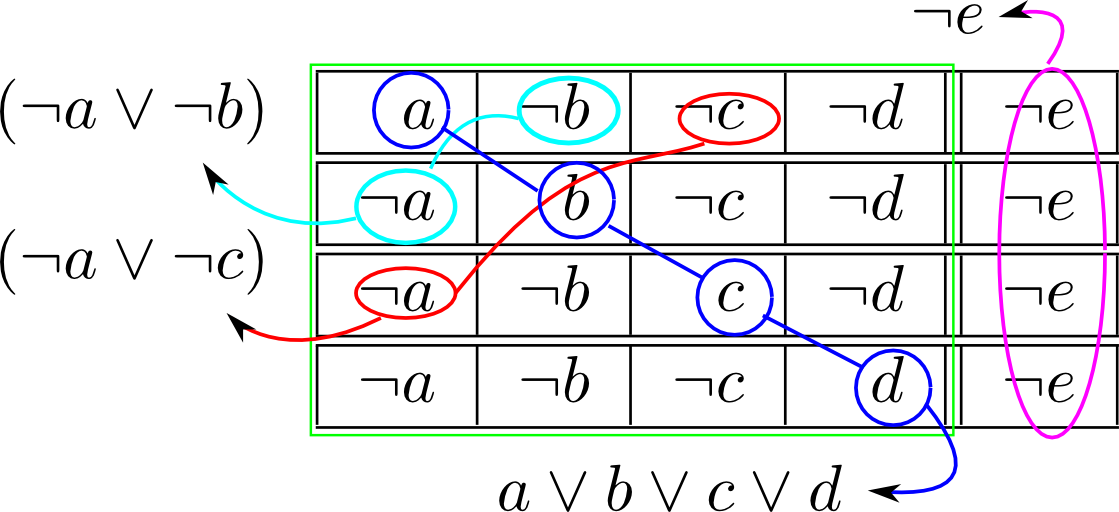
\includegraphics[scale=0.3]{generationFNC.png}
\caption{Génération de clauses}
\label{fig:generationFNC}
\end{figure}

Pour cette matrice, il est possible de formuler la contrainte en forme normale conjonctive suivante:
$$ (a \vee b \vee c \vee d ) \wedge (\lnot a \vee \lnot b) \wedge (\lnot a \vee \lnot c) \wedge (\lnot a \vee \lnot d)\wedge (\lnot b \vee \lnot c) \wedge (\lnot b \vee \lnot d)\wedge (\lnot c \vee \lnot d)$$   
À quoi, on ajoutera la clause unaire $\lnot e$.\\

Il est également à remarquer, comme sur la table \ref{table:tailleE}, que le nombre de clause représentant le nombre de colonne qui ne pourront jamais être une position $start$, est égal à:
\begin{itemize}
\item[]$\mathtt{L}(pos,ID) - 1$ pour une ligne 
\item[]$\mathtt{C}(pos,ID)-1$ pour une colonne
\end{itemize}  
	

\section{Représentation par bandes}
\subsection{Observation: position minimale, maximale et sous-espace}

Soit une colonne d'une longueur de 8 cases avec pour contrainte 3 bandes de taille 1, 2 et 1.

La première bande pourra prendre la position minimum $x_{1,0}$ et maximum $x_{1,\alpha}$.

La valeur de $\alpha$ peut être obtenue à partir du nombre de contraintes, de la taille des différentes bandes et de la règle selon laquelle deux bandes sont séparés d'au moins une case.\\

Dans l'exemple, on obtient:
\begin{itemize}
\item[] $c = 3$, où $c$ est le nombre de contraintes
\item[] $l = 8$ est la longueur de la colonne
\item[] $L_{total} = 4$, est la longueur cumulée des bandes dans la colonne
\item[] $\alpha = l-(L_{total}+(c-1))$
\end{itemize}

\begin{table}[H]
\centering
\begin{tabular}{|l||c|c|c|}
\hline 
0&\black • &  &  \\ 
\hline 
1 & &  &  \\ 
\hline 
2 & \grey &  & \black • \\ 
\hline 
3&\grey &  & \\ 
\hline 
4&\grey &  & \grey \\ 
\hline 
5&\grey &  & \grey \\ 
\hline 
6&\grey &  & \grey \\ 
\hline 
7&\grey &  & \grey \\ 
\hline &&\\
[-1.3em]\hline
&$min$ &  & $max$ \\ 
\hline 
\end{tabular} 
\caption{\label{bande8X1} position $max$ et $min$ sur une colonne $8\times1$ avec la contrainte 1 2 1}
\end{table}


On voit dans le tableau \ref{bande8X1} qu'il est possible de connaitre \textit{a priori} le nombre restreint de positions possibles pour la première bande. 

On voit aussi que chaque possibilité délimite un \textit{sous-espace} (zone grisée) au sein duquel devront être placées les bandes restantes.

Il est alors possible d'appliquer la même analyse quant à la détermination de la position de la bande suivante au sein du sous-espace.

Une fois les positions de la seconde bande déterminées, elles délimiteront l'espace restant pour la dernière bande. 

Suite à cela, il est possible d'élaborer une méthode récursive, ou faussement récursive, au nombre d'itérations réduit, permettant d'énumérer les possibilités de placement des bandes.

\subsection{Énumération récursive}
\begin{table}[H]
\centering
\begin{tabular}{|c|c|c|l|c|l|c|c|c|}
\hline 
\grey &&\black & \multicolumn{5}{l|}{$\updownarrow \mathtt{L}(1,1) = 1$}& $x_{1,1}=\top$ \\ 
\hline 
\grey && & \multicolumn{5}{l|}{+1} & $x_{1,2}=\bot$ \\ 
\hline
\grey &&\grey &  &  & \multicolumn{3}{l|}{$\#$ itération}& $x_{1,3}=\bot$ \\ 
\hline 
\grey &&\grey &  & \black - & \multicolumn{3}{l|}{$\updownarrow \mathtt{L}(1,2) = 2$}& $x_{1,4}=\top$ \\ 
\cline{1-5}\cline{9-9}
\grey &&\grey &  & \black - & \multicolumn{3}{l|}{}& $x_{1,5}=\top$\\ 
\hline 
\grey &&\grey &  &  & \multicolumn{3}{l|}{+1} & $x_{1,6}=\bot$\\ 
\hline 
\grey &&\grey &  & \grey &  & \black - & $\updownarrow \mathtt{L}(1,3) = 1$ & $x_{1,7}=\top$ \\ 
\hline 
\grey &&\grey &  & \grey &  &  &  & $x_{1,8}=\bot$\\ 
\hline
\hline 
 $\bullet$&&$r_1$ &  & $r_1$ &  &$r_3$&  \multicolumn{2}{c|}{récursion}\\
\hline
\end{tabular}
\caption{\label{EnumBande} Énumération récursive sur une colonne $8\times1$ avec la contrainte 1 2 1}
\end{table}

 
\begin{algorithm}
\caption{Énumération des bandes}
\begin{algorithmic}
\For{ligne $i \to n$}
		\For{colonne $j \to n$}
		nop();		
		\EndFor			
\EndFor
\end{algorithmic}
\end{algorithm}

	
						
\end{document}